%%%%%%%%%%%%%%%%%%%%%%%%%%%%%%%%%%%%%%%%%
% Structured General Purpose Assignment
% LaTeX Template
%
% Template Name: Anthony
% The template was named after my friend Anthony.
% Strong inspired by Apache Hadoop and Java (programming language)
%
% Author: Ang LEE
%
% Blog: http://angli.me/
%
% Github: https://github.com/leeang/
%
%%%%%%%%%%%%%%%%%%%%%%%%%%%%%%%%%%%%%%%%%

%----------------------------------------------------------------------------------------
%	CONSTANTS
%----------------------------------------------------------------------------------------

\newcommand{\hmwkTitle}{Report\ \#1}					% Assignment title
\newcommand{\hmwkClass}{Communication Networks}			% Course name
\newcommand{\hmwkClassTime}{}							% Workshop time
\newcommand{\hmwkClassInstructor}{}						% Tutor name
\newcommand{\hmwkAuthorName}{Ang LEE}					% Student name

\newcommand{\hmwkGraphicsPath}{img/}					% Graphics path
\newcommand{\hmwkCodePath}{code/}						% Code path

%----------------------------------------------------------------------------------------
%	TEMPLATE
%----------------------------------------------------------------------------------------

\documentclass{article}

\usepackage{fancyhdr}	% Required for custom headers
\usepackage{lastpage}	% Required to determine the last page for the footer
\usepackage{extramarks} % Required for headers and footers
\usepackage{graphicx}	% Required to insert images
\graphicspath{\hmwkGraphicsPath}
\usepackage{lipsum} 	% Used for inserting dummy 'Lorem ipsum' text into the template

\usepackage{float}
\usepackage{epstopdf}	% Required to insert .eps images
\usepackage{amssymb}
\usepackage{amsmath}
\usepackage[hidelinks]{hyperref}

% MATLAB syntax highlighting
\usepackage{color}		% Required to define colors
\definecolor{commentColor}{RGB}{34,139,34}
\definecolor{stringColor}{RGB}{160,32,240}
\usepackage{listings}
\lstset{
	inputpath=\hmwkCodePath,
	language=Matlab,
	basicstyle=\footnotesize\ttfamily,
	keywordstyle=\color{blue},
	stringstyle=\color{stringColor},
	commentstyle=\usefont{T1}{pcr}{m}{n}\color{commentColor},
	breaklines=true,
	showstringspaces=false
}

% Margins
\topmargin=-0.45in
\evensidemargin=0in
\oddsidemargin=0in
\textwidth=6.5in
\textheight=9.0in
\headsep=0.25in

\linespread{1.1}		% Line spacing

% Set up the header and footer
\pagestyle{fancy}
\lhead{\hmwkTitle} % Header Left 
\chead{\hmwkAuthorName} % Header Center
\rhead{\hmwkClass} % Header Right
\lfoot{\url{https://github.com/leeang/Communication-Networks}} % Footer Left
\cfoot{} % Footer Center
\rfoot{Page\ \thepage\ of\ \pageref{LastPage}} % Footer Right
\renewcommand\headrulewidth{0.4pt} % Size of the header rule
\renewcommand\footrulewidth{0.4pt} % Size of the footer rule

\setlength\parindent{0pt} % Removes all indentation from paragraphs

%----------------------------------------------------------------------------------------
%	Problem and Section
%----------------------------------------------------------------------------------------

\newenvironment{homeworkProblem}[1]{
	\section*{#1}
	}{
}
\newenvironment{homeworkSection}[1]{
	\subsection*{#1}
	}{
}
\newcommand{\problemAnswer}[1]{
	\noindent\framebox[\columnwidth][c]{
		\begin{minipage}{0.98\columnwidth}
			#1
		\end{minipage}
	}
}

%----------------------------------------------------------------------------------------
%	Document
%----------------------------------------------------------------------------------------

\begin{document}

\newpage

%----------------------------------------------------------------------------------------
%	PROBLEM 1.1
%----------------------------------------------------------------------------------------

\begin{homeworkProblem}{Question 1.1}
What are the main function groups in the window shown in Figure 1: Main Window of Wireshark 1.10?\\

Capture, Files, Online, Capture Help.
\end{homeworkProblem}

%----------------------------------------------------------------------------------------
%	PROBLEM 1.2
%----------------------------------------------------------------------------------------

\begin{homeworkProblem}{Question 1.2}
What are the four main uses of Wireshark? Which one applies to us?\\

Network administrators use it to troubleshoot network problems\\
Network security engineers use it to examine security problems\\
Developers use it to debug protocol implementations\\
People use it to learn network protocol internals\\

We use Wireshark to learn network protocol internals.\\

Reference:\\
\url{https://www.wireshark.org/docs/wsug_html_chunked/ChapterIntroduction.html#ChIntroPurposes}
\end{homeworkProblem}

%----------------------------------------------------------------------------------------
%	PROBLEM 1.3
%----------------------------------------------------------------------------------------

\begin{homeworkProblem}{Question 1.3}
Why is there a security link on the main window? List and explain with one sentence each of the two main security-related implications of using Wireshark.\\

In order to remind users to notice potential security vulnerabilities of Wireshark. In other words, to help users work with Wireshark as securely as possible.\\

\textbf{Don't run Wireshark as root/Administrator,} because using a root account makes any exploit far more dangerous: a successful exploit will have immediate control of the whole system, compromising it completely.\\

\textbf{Analyze capture files in an uncritical environment.} Users may create a special (limited) user account or even use a dedicated machine for this task, in case that breaches propagate in this computer or even in the whole network.\\

Reference: \url{https://wiki.wireshark.org/Security}
\end{homeworkProblem}

%----------------------------------------------------------------------------------------
%	PROBLEM 1.4
%----------------------------------------------------------------------------------------

\begin{homeworkProblem}{Question 1.4}
List the three different ways of selecting the ``Interface list'' functionality.\\

1. click interface list on the main windows\\
2. click Capture in the menu, then click Interfaces.\\
3. Ctrl + I
\end{homeworkProblem}

%----------------------------------------------------------------------------------------
%	PROBLEM 1.5
%----------------------------------------------------------------------------------------

\begin{homeworkProblem}{Question 1.5}
What is the ``promiscuous mode''? Describe what happens when Wireshark is in this mode?\\

Briefly, in promiscuous mode the MAC address filter is disabled and all packets of the currently joined network are captured.\\

If users are trying to capture network traffic that is not being sent to or from the machine running Wireshark or TShark, i.e. traffic between two or more other machines on an Ethernet segment, they will have to capture in ``promiscuous mode'', and, on a switched Ethernet network, they will have to set up the machine specially in order to capture that traffic.\\

In order to capture Ethernet traffic other than Unicast traffic to and from the host on which users are running Wireshark, Multicast traffic, and Broadcast traffic, the adapter will have to be put into promiscuous mode, so that the filter is switched off and all packets received are delivered to the host.\\

In addition, if users are on a switched Ethernet, rather than a shared Ethernet, users will also have to take action to ensure that all traffic in which users are interested is sent to the Ethernet adapter on the machine running the packet capture program; that is not, by default, the case on switched networks, so attempts to capture on a switched network will, by default, see only traffic that the capturing machine would see when not in promiscuous mode.\\

In the old days, Ethernet networks were shared networks, using shared media or hubs to connect the Ethernet nodes together, meaning all packets could be received by all nodes on that network. Therefore, if an Ethernet adapter on such a network is put into promiscuous mode, all packets on the network will be seen by that adapter and thus can be captured with that adapter.\\

Reference: \url{https://wiki.wireshark.org/CaptureSetup/Ethernet}
\end{homeworkProblem}

%----------------------------------------------------------------------------------------
%	PROBLEM 1.6
%----------------------------------------------------------------------------------------

\begin{homeworkProblem}{Question 1.6}
The string ``tcp port http'' is a Packet CAPture (PCAP) filter. What does this filter do?\\

An HTTP client initiates a request by establishing a TCP connection to a particular port on a server (typically port 80, occasionally port 8080).\\

If this filter is applied, only packets via TCP port 80 will be captured and saved, communication under other protocols will be ignored.
\end{homeworkProblem}

%----------------------------------------------------------------------------------------
%	PROBLEM 1.7
%----------------------------------------------------------------------------------------

\begin{homeworkProblem}{Question 1.7}
Observe that the main window has three main horizontal content segments (other than toolbars and menus). Describe each with a sentence.\\

The \textbf{packet list pane} displays all the packets in the current capture file.\\
The \textbf{packet details pane} shows the current packet (selected in the ``Packet List'' pane) in a more detailed form.\\
The \textbf{packet bytes pane} shows the data of the current packet (selected in the ``Packet List'' pane) in a hexdump style.\\

Reference:\\
\url{https://www.wireshark.org/docs/wsug_html_chunked/ChUsePacketListPaneSection.html}\\
\url{https://www.wireshark.org/docs/wsug_html_chunked/ChUsePacketDetailsPaneSection.html}\\
\url{https://www.wireshark.org/docs/wsug_html_chunked/ChUsePacketBytesPaneSection.html}
\end{homeworkProblem}

%----------------------------------------------------------------------------------------
%	PROBLEM 2.1
%----------------------------------------------------------------------------------------

\begin{homeworkProblem}{Question 2.1}
Describe the difference between the capture and display filters with a sentence.\\

Basically capture filters work while capturing, display filters work while viewing.\\

If the capture filter is applied, only interested packets will be captured and saved. Sometimes, users want to keep information as detailed as possible and thus save a host of data. However, it becomes hard to find the packets that users are really concerned about. Display filter will help users filter irrelevant packets. 
\end{homeworkProblem}

%----------------------------------------------------------------------------------------
%	PROBLEM 2.2
%----------------------------------------------------------------------------------------

\begin{homeworkProblem}{Question 2.2}
What are the IP and MAC addresses of the client computer (where browser is) and the server?\\

Client IP: 192.168.0.5\\
Server IP: 50.23.66.4\\

Client MAC: 00:24:1d:77:8d:6d\\
Server MAC: 08:bd:43:61:50:87
\end{homeworkProblem}

%----------------------------------------------------------------------------------------
%	PROBLEM 2.3
%----------------------------------------------------------------------------------------

\begin{homeworkProblem}{Question 2.3}
Describe the communication between the browser and server at the http level. What do ``GET'' and ``200 OK'' mean in HTTP which you use every day? (Your answer should be short, preferably couple of sentences).\\

\textbf{Description}\\
A client sends a request to the server in the form of a request method, URI, and protocol version, followed by a MIME-like message containing request modifiers, client information, and possible body content over a connection with a server. The server responds with a status line, including the message's protocol version and a success or error code, followed by a MIME-like message containing server information, entity metainformation, and possible entity-body content.\\

Reference: \url{http://www.w3.org/Protocols/rfc2616/rfc2616-sec1.html}\\

\textbf{GET}\\
The GET method means retrieve whatever information (in the form of an entity) is identified by the Request-URI. If the Request-URI refers to a data-producing process, it is the produced data which shall be returned as the entity in the response and not the source text of the process, unless that text happens to be the output of the process.\\

Reference: \url{http://www.w3.org/Protocols/rfc2616/rfc2616-sec9.html}\\

\textbf{200 OK}\\
``200 OK'' is a HTTP status code which means the request has succeeded. In a GET request, an entity corresponding to the requested resource is sent in the response.\\

Reference: \url{http://www.w3.org/Protocols/rfc2616/rfc2616-sec10.html}
\end{homeworkProblem}

%----------------------------------------------------------------------------------------
%	PROBLEM 2.4
%----------------------------------------------------------------------------------------

\begin{homeworkProblem}{Question 2.4}
What was the title of the webpage?\\

Test Page for Wireshark Workshop
\end{homeworkProblem}

%----------------------------------------------------------------------------------------
%	PROBLEM 2.5
%----------------------------------------------------------------------------------------

\begin{homeworkProblem}{Question 2.5}
Note that, some of the ARP packets in the trace are described as ``Gratuitous\_ARP''. What is a ``Gratitious ARP'' and why is it used?\\

Gratuitous ARP could mean both gratuitous ARP request or gratuitous ARP reply. Gratuitous in this case means a request/reply that is not normally needed according to the ARP specification (RFC 826) but could be used in some cases. A gratuitous ARP request is an AddressResolutionProtocol request packet where the source and destination IP are both set to the IP of the machine issuing the packet and the destination MAC is the broadcast address ff:ff:ff:ff:ff:ff. Ordinarily, no reply packet will occur. A gratuitous ARP reply is a reply to which no request has been made.\\

Gratuitous ARPs are useful for four reasons:\\

1. They can help detect IP conflicts. When a machine receives an ARP request containing a source IP that matches its own, then it knows there is an IP conflict.\\

2. They assist in the updating of other machines' ARP tables. Clustering solutions utilize this when they move an IP from one NIC to another, or from one machine to another. Other machines maintain an ARP table that contains the MAC associated with an IP. When the cluster needs to move the IP to a different NIC, be it on the same machine or a different one, it reconfigures the NICs appropriately then broadcasts a gratuitous ARP reply to inform the neighboring machines about the change in MAC for the IP. Machines receiving the ARP packet then update their ARP tables with the new MAC.\\

3. They inform switches of the MAC address of the machine on a given switch port, so that the switch knows that it should transmit packets sent to that MAC address on that switch port.\\

4. Every time an IP interface or link goes up, the driver for that interface will typically send a gratuitous ARP to preload the ARP tables of all other local hosts. Thus, a gratuitous ARP will tell us that that host just has had a link up event, such as a link bounce, a machine just being rebooted or the user/sysadmin on that host just configuring the interface up. If we see multiple gratuitous ARPs from the same host frequently, it can be an indication of bad Ethernet hardware/cabling resulting in frequent link bounces.\\

Referrence: \url{https://wiki.wireshark.org/Gratuitous_ARP}
\end{homeworkProblem}

%----------------------------------------------------------------------------------------
%	PROBLEM 3.1
%----------------------------------------------------------------------------------------

\begin{homeworkProblem}{Question 3.1}
What does the CSV file contain? Does it contain the packet contents?\\

The CSV file contains 7 fields: No., Time, Source, Destination, Protocol, Length and Info.\\
It does not contain packet contents.
\end{homeworkProblem}

%----------------------------------------------------------------------------------------
%	PROBLEM 3.2
%----------------------------------------------------------------------------------------

\begin{homeworkProblem}{Question 3.2}
Compute the sequence of packet inter-arrival times (IAT), i.e. the `gap' times between packets. Give simple statistics about this time series: minimum, maximum, average, standard deviation.\\

minimum: 0.000000\\
maximum: 16.902741\\
average: 0.005212\\
standard deviation: 0.204404
\end{homeworkProblem}

%----------------------------------------------------------------------------------------
%	PROBLEM 3.3
%----------------------------------------------------------------------------------------

\begin{homeworkProblem}{Question 3.3}
`Clean' the time series by selecting the subset of inter-arrival times smaller than the 95-th percentile. Use this subset as the time series for the next questions. Comment on the statistics of this cleaned series: minimum, maximum, average, standard deviation.\\

minimum (clean): 0.000000\\
maximum (clean): 0.006475\\
average (clean): 0.001071\\
standard deviation (clean): 0.001189
\end{homeworkProblem}

%----------------------------------------------------------------------------------------
%	PROBLEM 3.4
%----------------------------------------------------------------------------------------

\begin{homeworkProblem}{Question 3.4}
Plot the time series and histogram of the cleaned packet inter-arrival times (IATs). Add a title, label the X and Y axis with correct units. Include the figure in your report.\\

Histogram will be shown in Question 3.6 together with exponential trend line.

\begin{figure}[H]
\centering
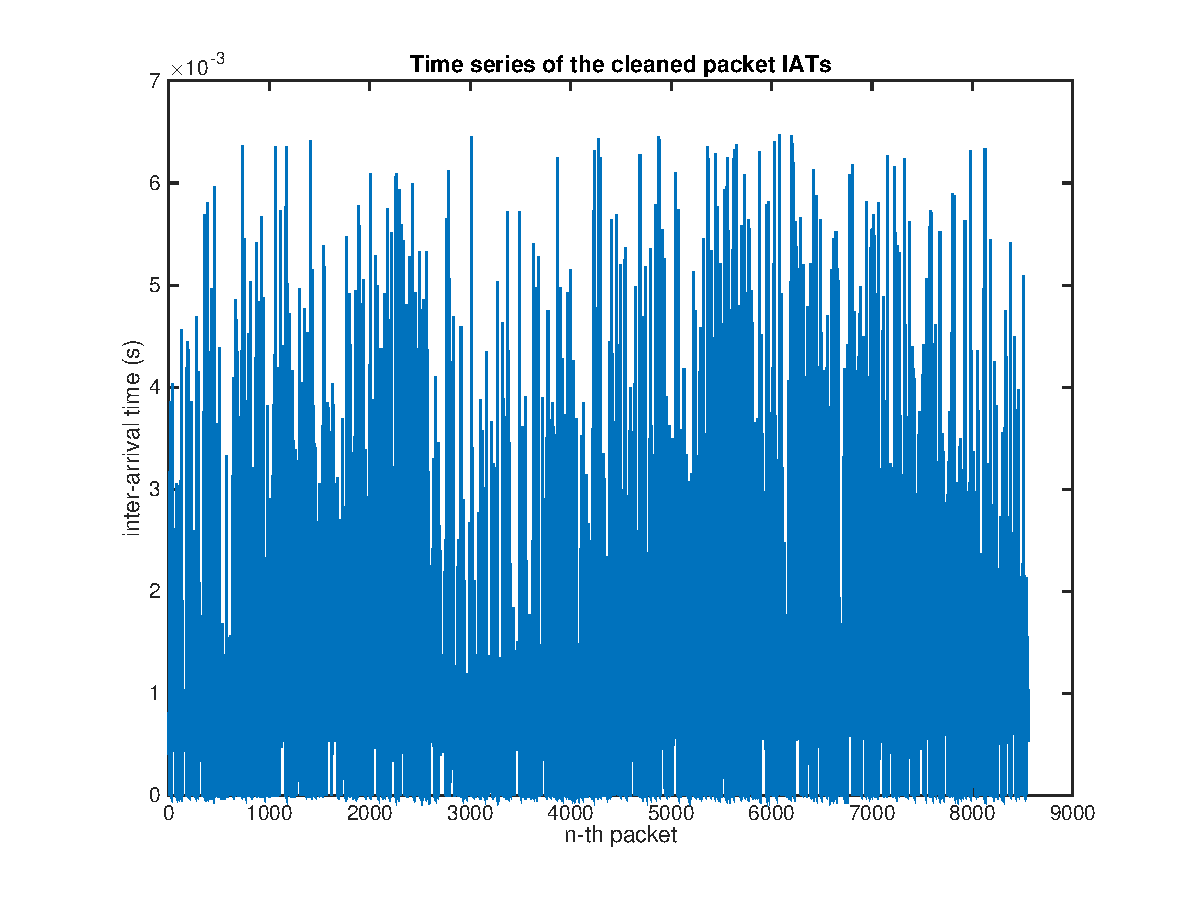
\includegraphics[width=6.6in]{img/time-series1.eps}
\caption{Time series of the cleaned packet IATs}
\end{figure}

\end{homeworkProblem}

%----------------------------------------------------------------------------------------
%	PROBLEM 3.5
%----------------------------------------------------------------------------------------

\begin{homeworkProblem}{Question 3.5}
Using the expfit function, try to fit an exponential law to the distribution of the (inter-arrival) time series.\\

Exponential parameter = 0.0011
\end{homeworkProblem}

%----------------------------------------------------------------------------------------
%	PROBLEM 3.6
%----------------------------------------------------------------------------------------

\begin{homeworkProblem}{Question 3.6}
Plot the packet IAT distribution and superimpose the exponential distribution obtained with expfit. Include the figure in your report. Would you agree with the following statement for the packets captured?\\
``the packet arrival time series can be accurately modelled by a Poisson process''?\\

Argue the case for or against the statement. Note that the answer may well be negative! Please focus on your reasoning and showing your understanding, not the simple answer.\\

\begin{figure}[H]
\centering
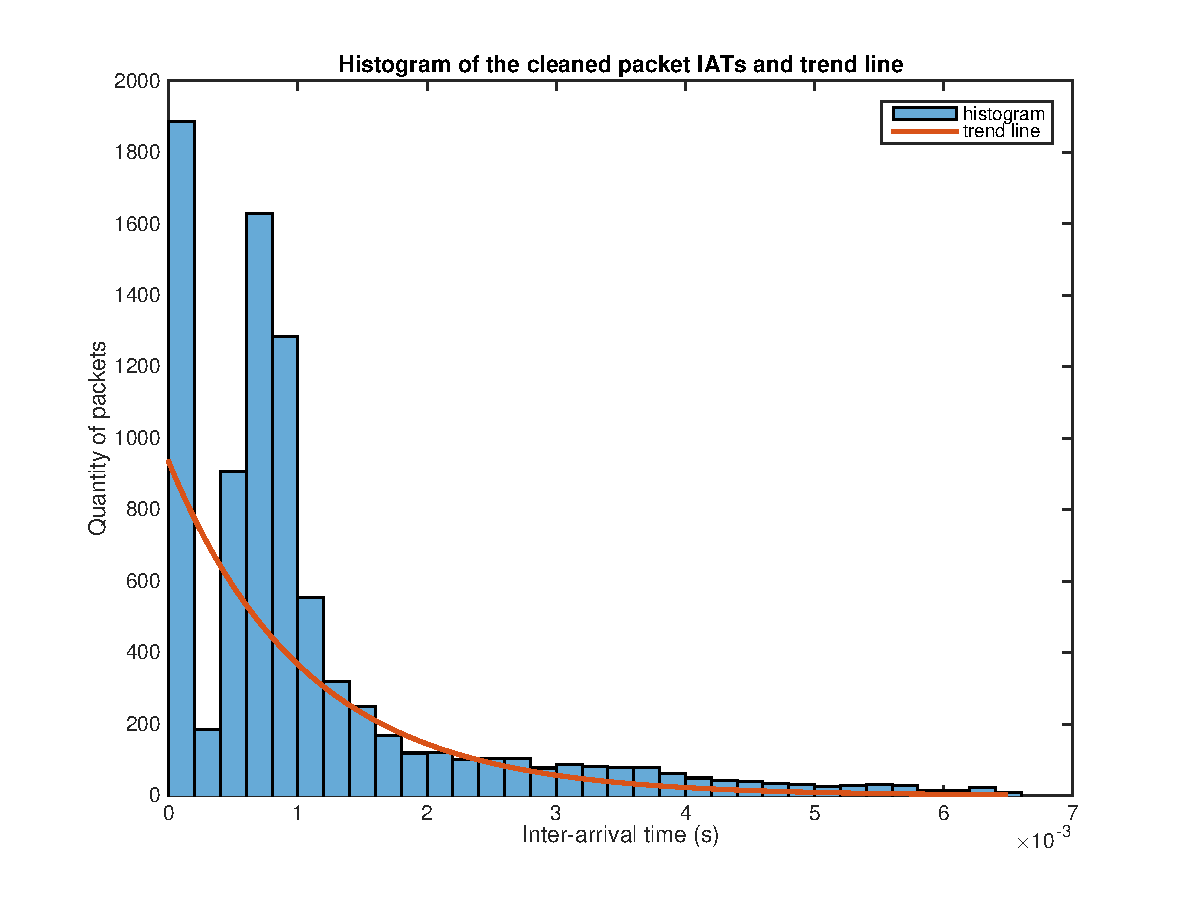
\includegraphics[width=6.6in]{img/histogram1.eps}
\caption{Histogram of the cleaned packet IATs and trend line}
\end{figure}
\end{homeworkProblem}

No, the packet arrival time series cannot be accurately modelled by a Poisson process.\\

As is well known, Poisson process primarily makes two assumptions: 1. The number of sources is infinite; 2. The traffic arrival pattern is random. Apparently, the first condition does not hold at current circumstance. After the view filter applied, only packets from a certain server to my laptop were taken into consideration. Besides, communication via Wide area network will also introduce some regular influence (not totally random). If Wireshark was run on a web server and analyzed packets from different IP addresses , the exponential regression would be more accurate. In addition, insufficiency of specimen (sample time $\approx$ 1 min) had negative impact on accuracy as well.

%----------------------------------------------------------------------------------------
%	Bonus
%----------------------------------------------------------------------------------------
\clearpage
\begin{homeworkProblem}{Question 3.2 Bonus}
Compute the sequence of packet inter-arrival times (IAT), i.e. the `gap' times between packets. Give simple statistics about this time series: minimum, maximum, average, standard deviation.\\

\textbf{Data Set 2}\\
minimum: 0.000001\\
maximum: 30.307905\\
average: 0.030534\\
standard deviation: 0.849335\\

\textbf{Data Set 3}\\
minimum: 0.000000\\
maximum: 9.012183\\
average: 0.010091\\
standard deviation: 0.232632
\end{homeworkProblem}

\begin{homeworkProblem}{Question 3.3 Bonus}
`Clean' the time series by selecting the subset of inter-arrival times smaller than the 95-th percentile. Use this subset as the time series for the next questions. Comment on the statistics of this cleaned series: minimum, maximum, average, standard deviation.\\

\textbf{Data Set 2}\\
minimum (clean): 0.000001\\
maximum (clean): 0.002141\\
average (clean): 0.000781\\
standard deviation (clean): 0.000311\\

\textbf{Data Set 3}\\
minimum (clean): 0.000000\\
maximum (clean): 0.003212\\
average (clean): 0.000908\\
standard deviation (clean): 0.000650
\end{homeworkProblem}

\begin{homeworkProblem}{Question 3.4 Bonus}
Plot the time series and histogram of the cleaned packet inter-arrival times (IATs). Add a title, label the X and Y axis with correct units. Include the figure in your report.\\

Histogram will be shown in Question 3.6 together with exponential trend line.

\begin{figure}[H]
\begin{minipage}[t]{0.5\linewidth}
\centering
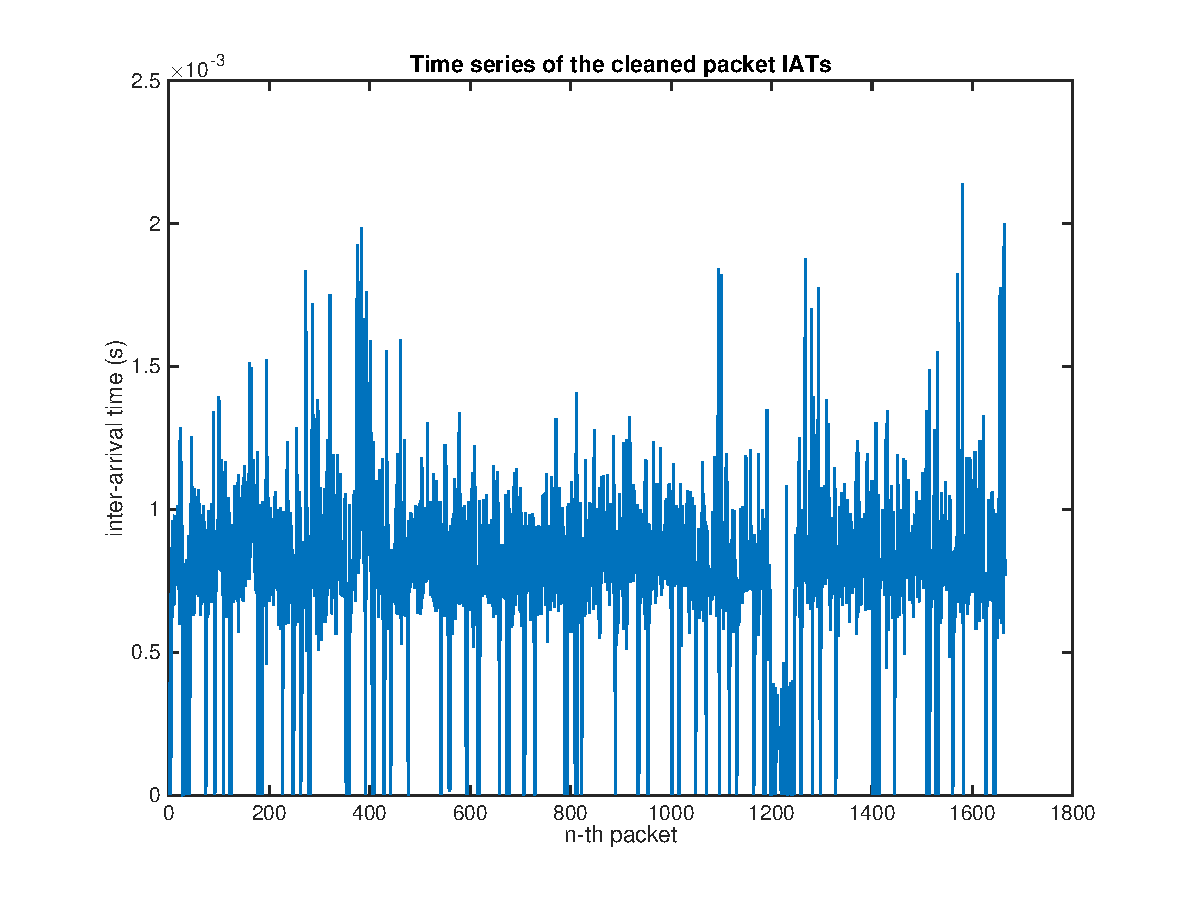
\includegraphics[width=3.3in]{img/time-series2.eps}
\caption{Time series (Data Set 2)}
\end{minipage}
\begin{minipage}[t]{0.5\linewidth}
\centering
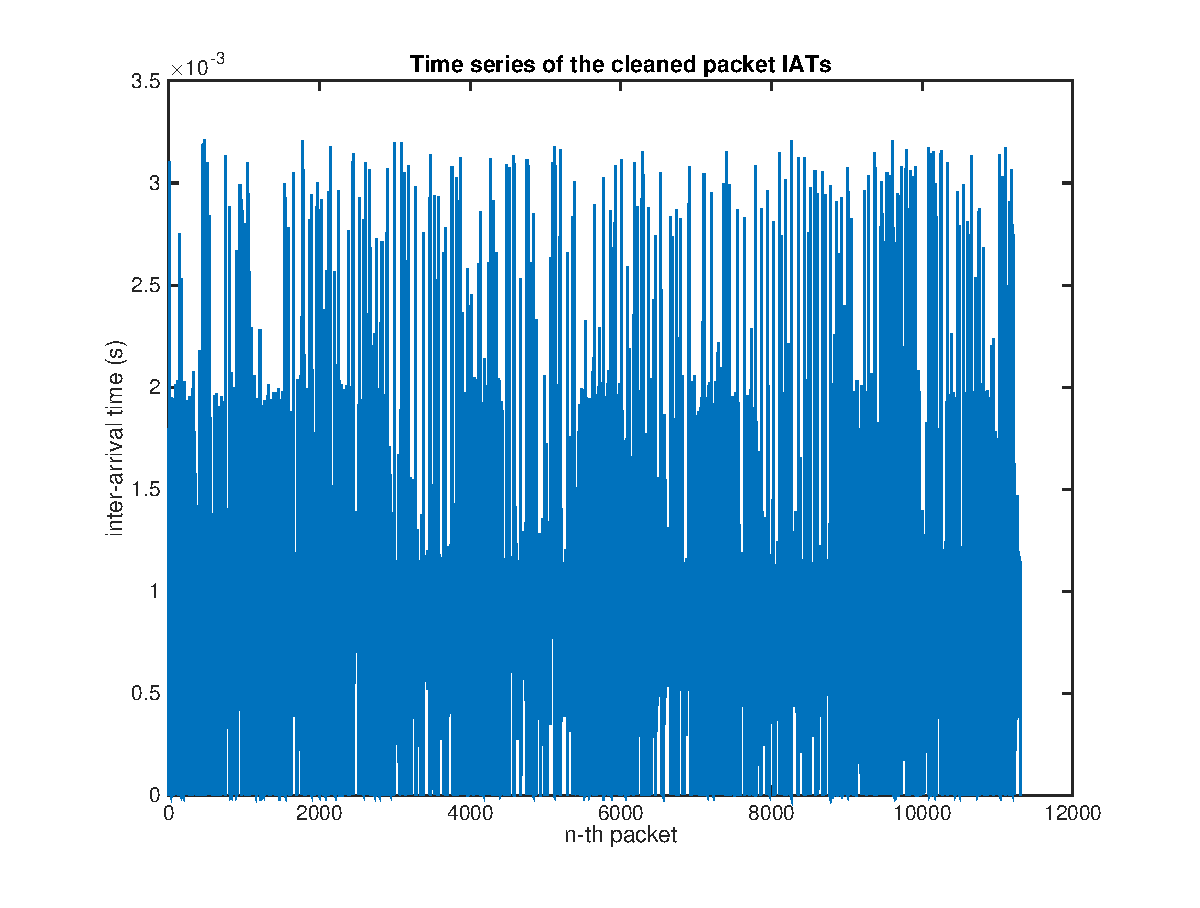
\includegraphics[width=3.3in]{img/time-series3.eps}
\caption{Time series (Data Set 3)}
\end{minipage}
\end{figure}

\end{homeworkProblem}

\begin{homeworkProblem}{Question 3.5 Bonus}
Using the expfit function, try to fit an exponential law to the distribution of the (inter-arrival) time series.\\

\textbf{Data Set 2}\\
Exponential parameter = 7.8087e-04\\

\textbf{Data Set 3}\\
Exponential parameter = 9.0753e-04
\end{homeworkProblem}

\begin{homeworkProblem}{Question 3.6 Bonus}
Plot the packet IAT distribution and superimpose the exponential distribution obtained with expfit. Include the figure in your report. Would you agree with the following statement for the packets captured?\\

\begin{figure}[H]
\begin{minipage}[t]{0.5\linewidth}
\centering
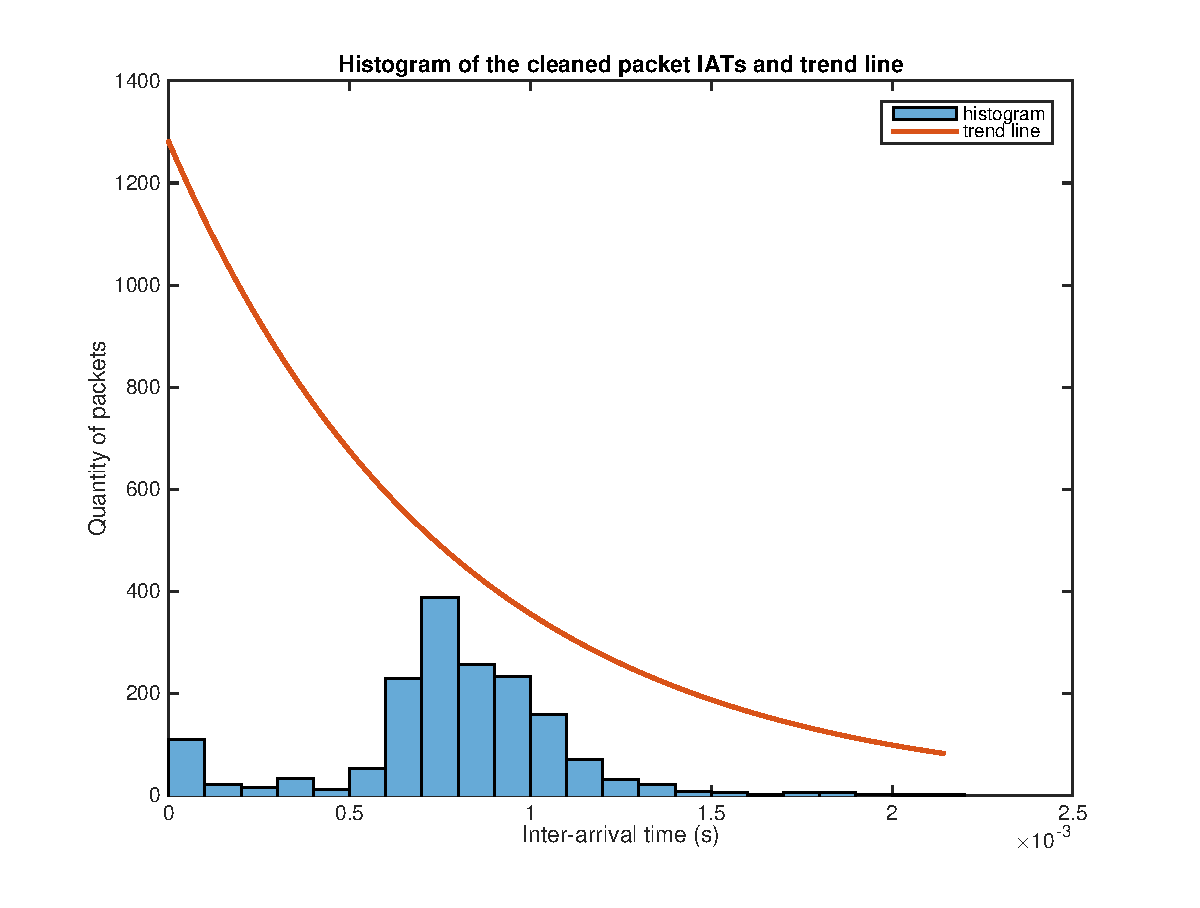
\includegraphics[width=3.3in]{img/histogram2.eps}
\caption{Histogram and trend line (Data Set 2)}
\end{minipage}
\begin{minipage}[t]{0.5\linewidth}
\centering
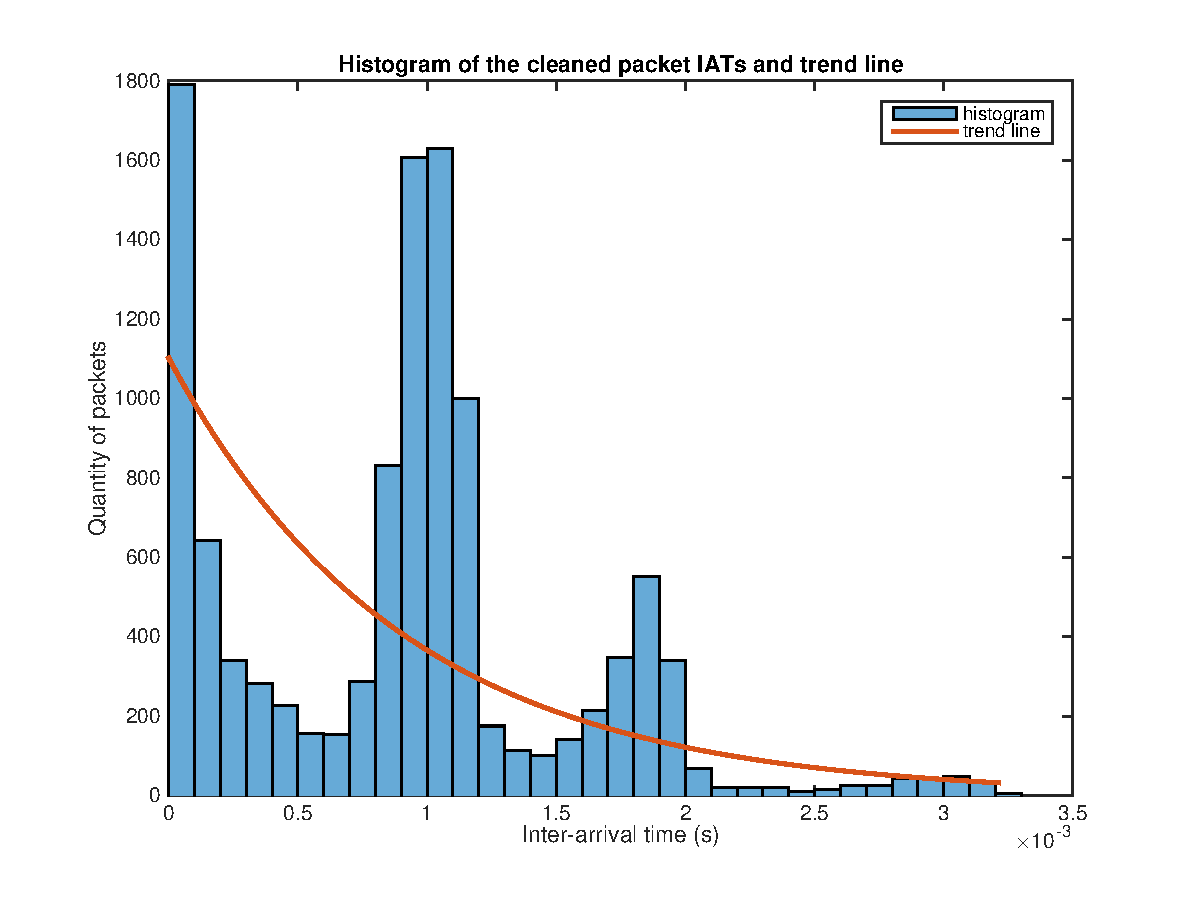
\includegraphics[width=3.3in]{img/histogram3.eps}
\caption{Histogram and trend line (Data Set 3)}
\end{minipage}
\end{figure}
\end{homeworkProblem}

\begin{homeworkProblem}{Question 3.7 Bonus}
In order to make data set 2 and 3 various, we sampled for longer period ($\approx$ 3 min) or utilized another laptop respectively.\\

A Poisson process has following properties: The time between two subsequent arrivals has an Exponential distribution; For any two disjoint intervals, the number of visits in each are independent of each other. Both histograms look far different from exponential distribution. Hence, the packet arrival time series cannot be modeled by a Poisson distribution. (From ELEN90054 Probability and Random Models)\\

Due to network latency, cache mechanism, Border Gateway Protocol (announcing the same destination IP address from many different places on the Internet) etc., independent disjoint intervals turn out to be impractical. This point could be another reason for the failure of Poisson model.\\

Interestingly, the histogram of data set 2 looks like Normal distribution (shown below). Probably, after plenty of hops (passing through bridges, routers and gateways), normal distribution covers up the underlying distribution.\\

``In probability theory, the central limit theorem (CLT) states that, given certain conditions, the arithmetic mean of a sufficiently large number of iterates of independent random variables, each with a well-defined expected value and well-defined variance, will be approximately normally distributed, regardless of the underlying distribution.''

\begin{figure}[H]
\centering
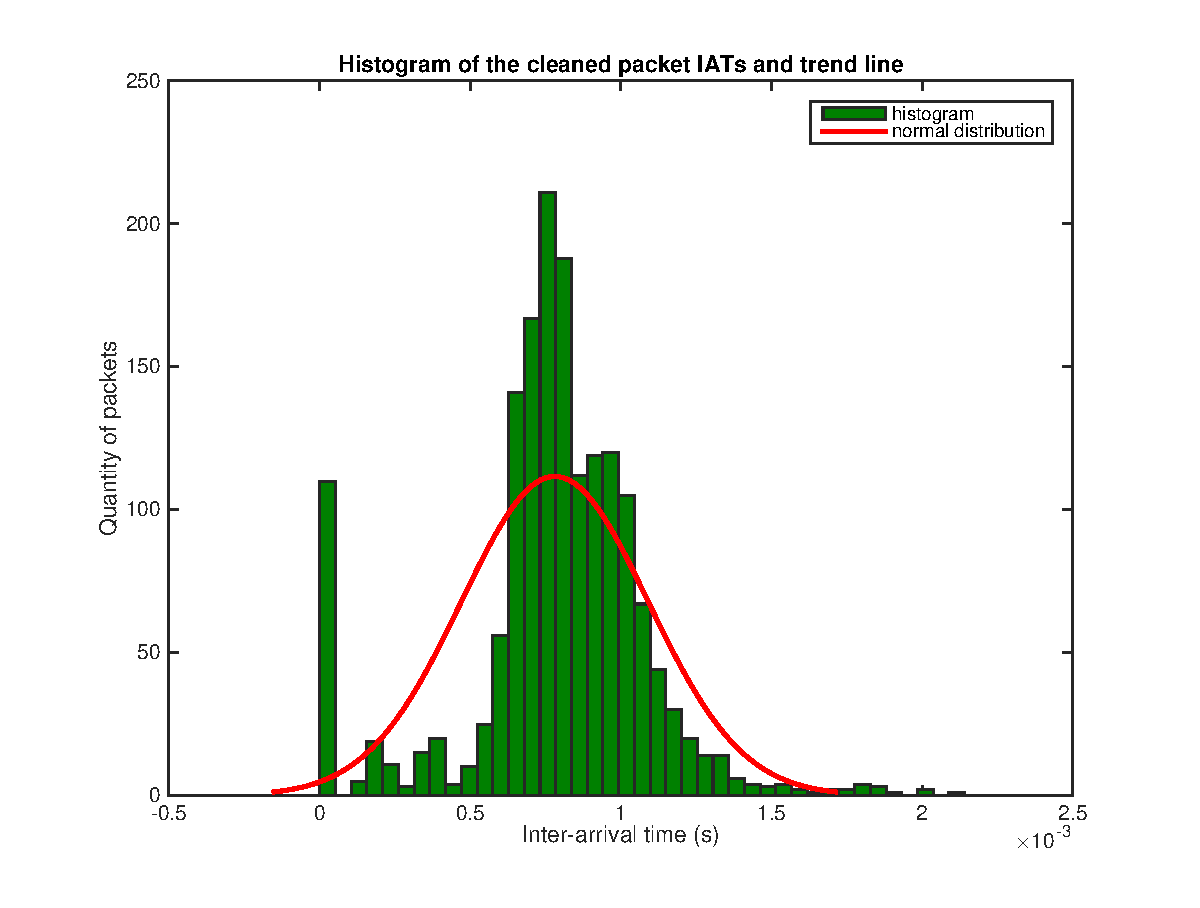
\includegraphics[width=6in]{img/histogram2-normal.eps}
\caption{Histogram and normal distribution trend line (Data Set 3)}
\end{figure}
\end{homeworkProblem}

%----------------------------------------------------------------------------------------

\clearpage

%----------------------------------------------------------------------------------------
%	Appendix
%----------------------------------------------------------------------------------------

\begin{homeworkProblem}{Appendix}

%--------------------------------------------

\begin{homeworkSection}{Question 3 MATLAB code}

\problemAnswer{
	\lstinputlisting{workshop1.m}
}

\end{homeworkSection}

%--------------------------------------------

\end{homeworkProblem}

%----------------------------------------------------------------------------------------

\end{document}
